\chapter{Sluneční skvrny}

\section{Vznik slunečních skvrn}
S magnetickým polem je spojena sluneční aktivita, jako sluneční erupce, výrony koronální hmoty a sluneční skvrny. V důsledku konvektivních pohybů a diferenciální rotace není magnetické pole Slunce čistě dipólové. Jeho deformace se v celkovém součtu vyruší a z velké vzdálenosti má pole charakter dipólu, ale lokálně se projevují sluneční aktivitou. Magnetické pole v elektricky nabitém plynu doprovází magnetický tlak. V případě, že magnetická silotrubice vystoupí to fotosféry, dojde v místech, kde silotrubice vystupuje nad povrch ke snížení tlaku plynu, aby tlak plynu a magnetický tlak byl v součtu stejný, jako tlak v okolí. Oblasti s nízkým tlakem se začnou ochlazovat a v důsledku toho vznikají místa s nižší teplotou (\unit[3000-4000]{K} oproti \unit[5000-6000]{K} ve zbytku fotosféry).

Místa, kde silotrubice vystupuje do fotosféry jsou tedy chladnější a mají mnohonásobně (cca 4-5krát) menší zářivý výkon než okolí a pozorujeme je jako tmavá. V souladu s charakterem jejich původu pozorujeme sluneční skvrny ve většině případů v páru, jelikož silotrubice musí fotosféru protnout ve dvou místech. Typické rozměry slunečních skvrn se pohybují mezi $\unit[3500-60000]{km}$.

Přesný mechanismus a příčiny pro výstup silotrubice do fotosféry ovšem stále nejsou zcela objasněny.


\section{Struktura slunečních skvrn}

\subsection{Wilsonova deprese}
Pro sluneční skvrny je optické hloubky $\tau=1$ dosaženo ve větší hloubce, než v klidném Slunci (zhruba o $\unit[0.5-2]{Mm}$ hlouběji). Znamená to tedy, že fotony mající původ ve slunčení skvrně, které opustí Slunce jsou produkovány v průměrně větší hloubce, než fotony, které vidíme ze zbytku fotosféry. Tento jev se nazývá Wilsonova deprese.

Důvodem je nížší teplota a tlak plynu, než je v okolí, což má za následek snížení opacity, která s optickou hloubkou přímo souvisí.

\subsection{Jemná struktura}
Nejvýraznějšími částmi sluneční skvrny jsou \textit{umbrální jádro} a \textit{penumbra}. Umbra je jádro sluneční skvrny. Je její nejchladnější a nejtmavší částí. Umbrální jádro obklopuje penumbra, která se skládá z protáhlých, převážně radiálně orientovaných struktur. Ty jsou důsledkem odklonu magnetického pole od kolmice v okolí umbrálního jádra. Teplota penumbry je již výrazně vyšší, než teplota umbrálního jádra; dosahuje hodnot pouze zhruba o $\unit[250-400]{K}$ nižších než je teplota okolí.

V umbrálním jádře jsou pozorovány světlé body, zvané \textit{umbrální body}. Jsou projevem konvekce uvnitř sluneční skvrny a dokazují, že zde stále dochází ke konvektivnímu přenosu energie. Světlé struktury, které z vnějšku zasahují do jádra, či od sebe 2 jádra oddělují se nazývají \textit{světelné mosty}. Jsou projevem silné konvekce a vznikají při zániku slunečních skvrn z umbrálních bodů. Struktura sluneční skvrny je znázorněna na obr. \ref{fig:skvrna}

\begin{figure}[h!]
	\centering
	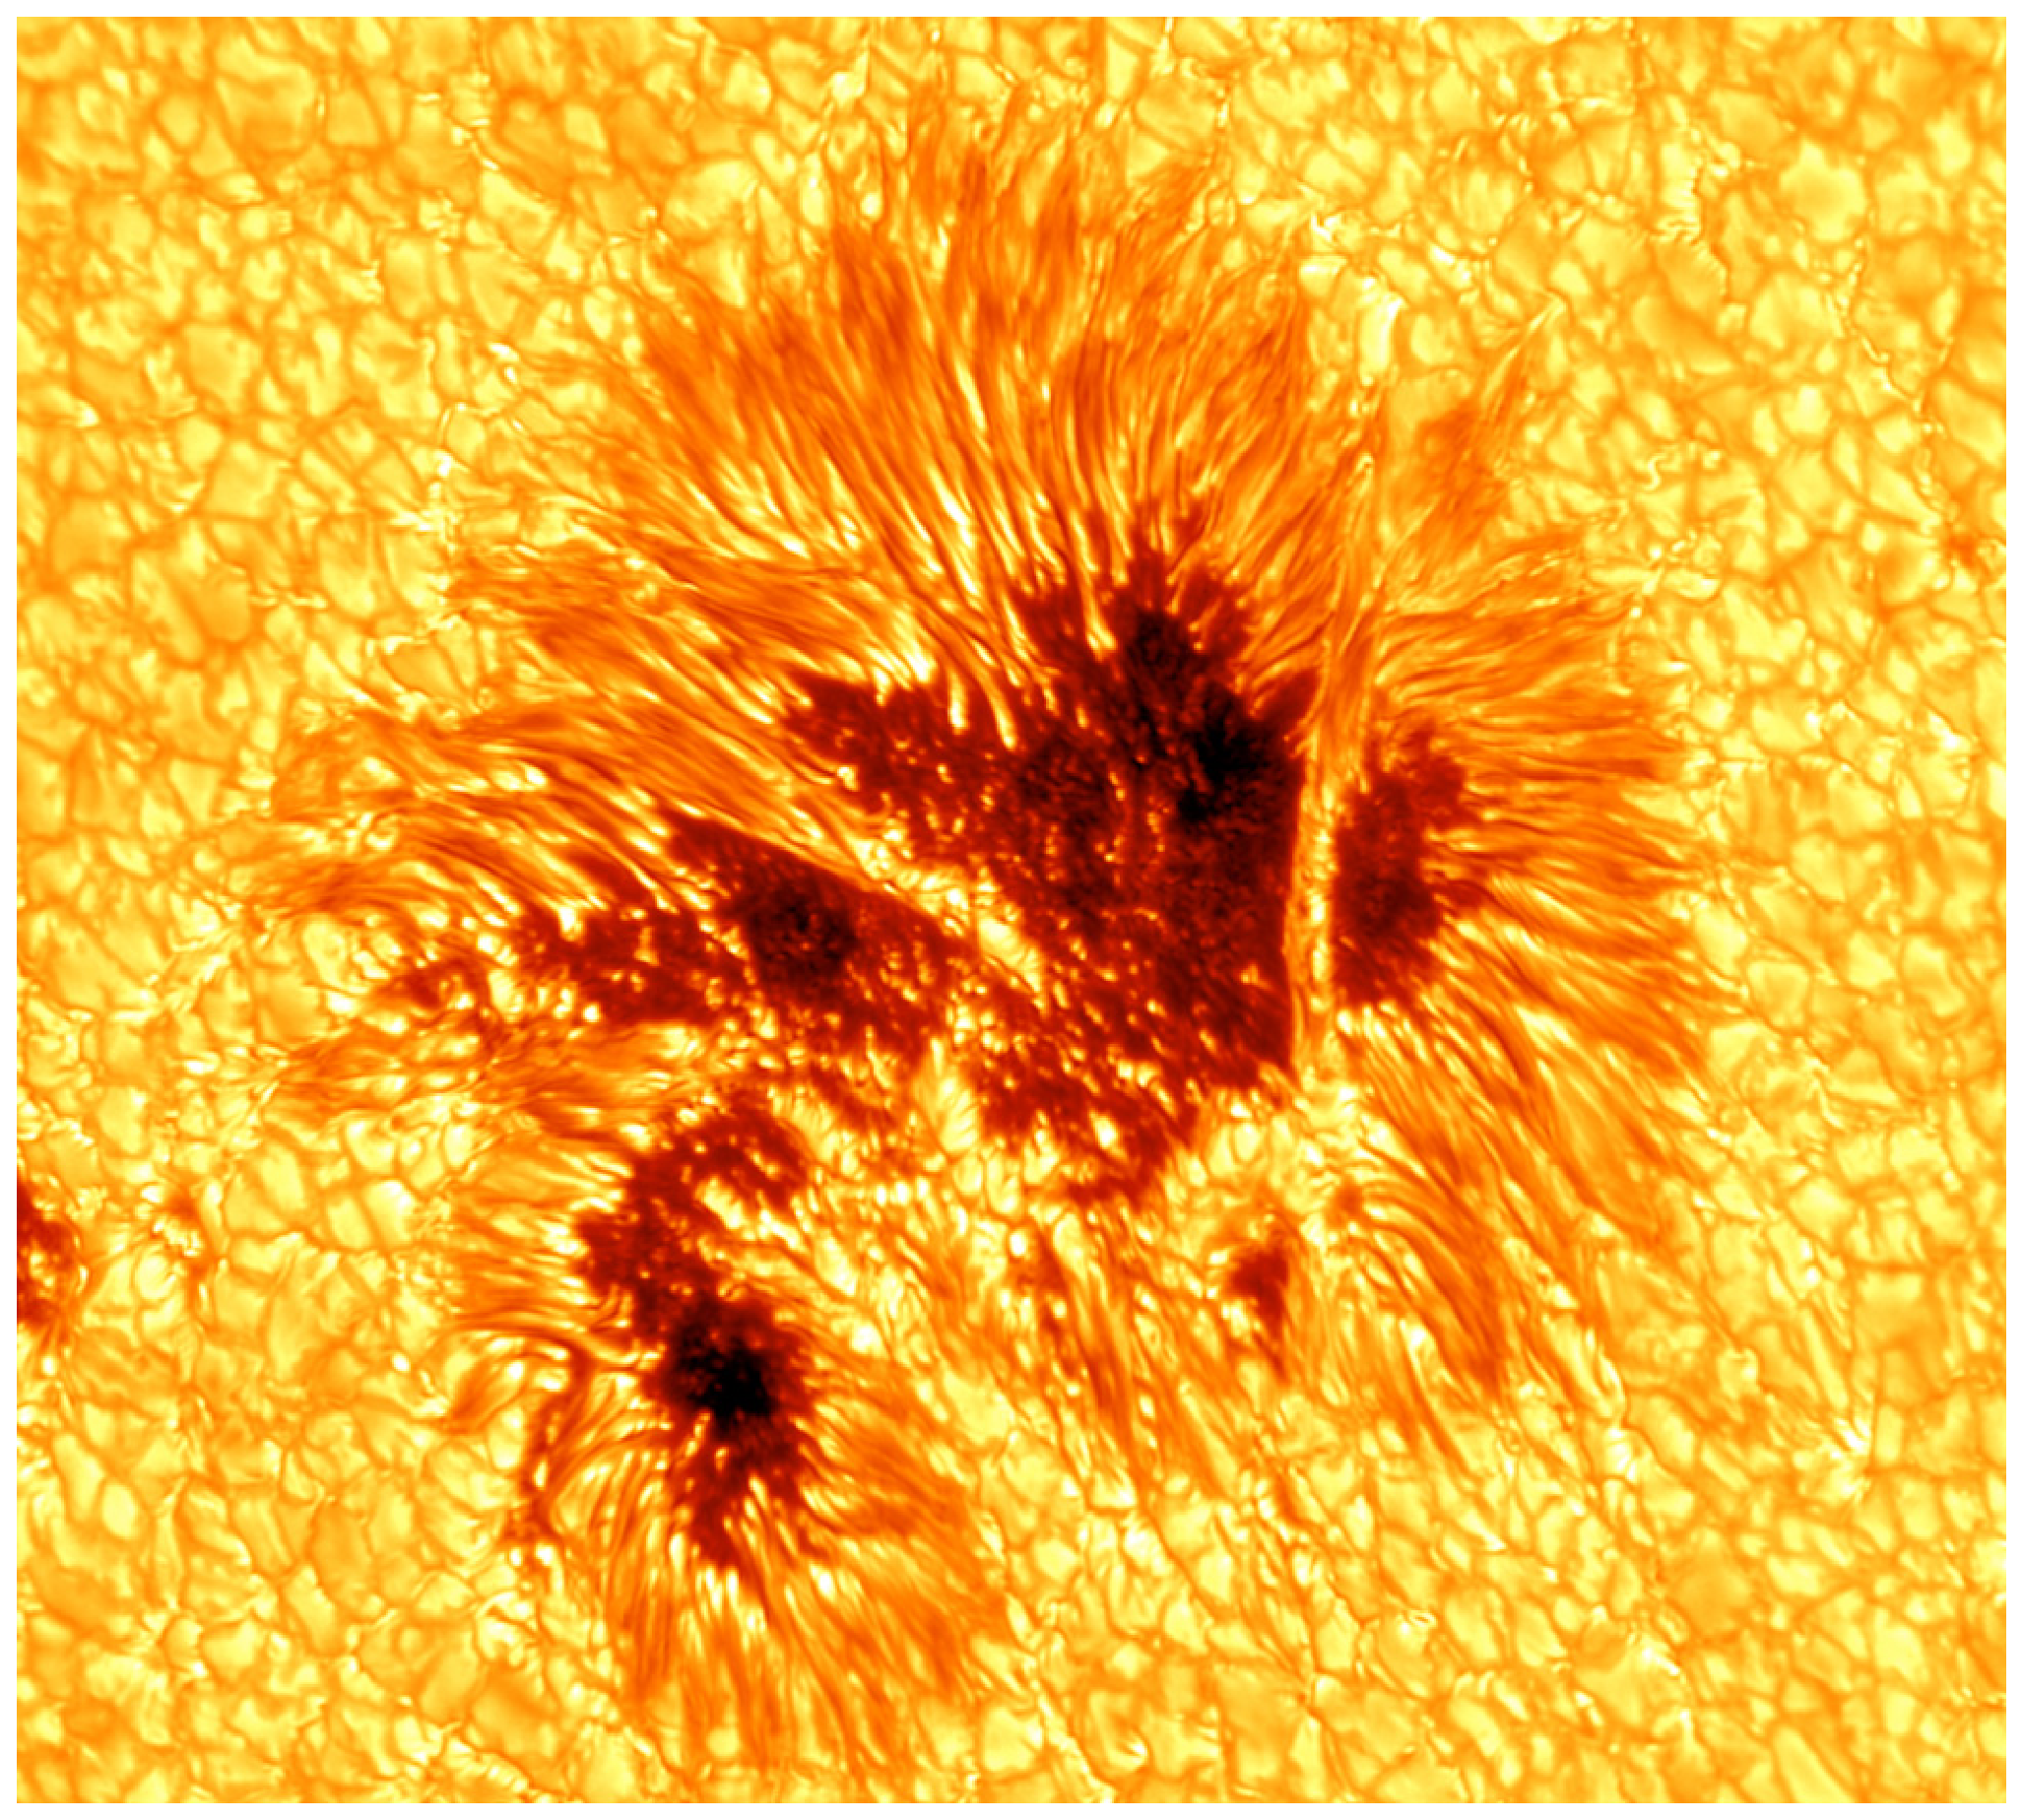
\includegraphics[scale=0.2]{../img/sunspot_structure.eps}
	\caption{zdroj: \url{http://www.extremetech.com/extreme/163460-marvel-at-the-most-detailed-photos-of-the-sun-ever-taken}}
	\label{fig:stavba}
\end{figure}


\section{Teoretické modely slunečních skvrn}
Všechny modely slunečních skvrn předpokládají, že skvrna je tvořena jednou osově symetrickou silotrubicí a ve většině modelů je soustava v magnetohydrostatické rovnováze, která je předepsána rovnováhou mezi silami uvnitř a vně silotrubice a Maxwellovou rovnicí:
\begin{align}
	\frac{1}{\mu_0}(\nabla\times\vect{B})\times\vect{B} &= \nabla p-\rho\vect{g} \label{eq:mh_equilib} \\
	\nabla\cdot\vect{B} &= 0
\end{align}
Předpoklad, že soustava je v každém okamžiku v hydrostatické rovnováze je většinou oprávněná, neboť vývoj slunečních skvrn probíhá v mnohem delších časových škálách, než je doba, po jakou se šíří vzruchy napříč silotrubicí.

\subsection{Self-similar modely}
Self-similar řešení jsou založena na předpokladu, že magnetické pole není zakroucené (tedy $B_\theta(r,z)=0$) a radiální závislost $\vect{B}$ je v každé hloubce stejná až na škálovací faktor, který zajišťuje konstantní magnetický tok při rozšiřování, nebo zužování silotrubice. Předpokládá se tedy následující:
\begin{equation}
	B_z(r,z)=f(\zeta)B_0(z),
	\label{eq:Bz}
\end{equation}
kde $B_0(z)$ je intenzita magnetického pole na ose symetrie, $\zeta=r\sqrt{B_0(z)}$ a $f(\zeta)$ je funkce určující tvar závislosti. Z Maxwellovy rovnice pro divergenci magnetického pole lze poté odvodit:
\begin{equation}
	B_r(r,z)=-rf(\zeta)\frac{\D B_0(z)}{\D z}
	\label{eq:Br}
\end{equation}
Pro zachování konstantního magnetického toku $\Phi$ silotrubicí je na funkci $f(\zeta)$ kladena podmínka
\begin{equation}
	2\pi\int\limits_0^{+\infty}f(\zeta)\zeta\,\D\zeta=\Phi.
\end{equation}
Je zvykem volit jako $f(\zeta)=\exp(-\zeta^2)$, která tuto podmínku splňuje.

Problém self-similar modelů může být, že jsou na magnetické pole kladeny příliš silné předpoklady. V modelech není skvrna vidět jako umbrální jádro obklopené penumbrou. Důkladnější modely také ukazují, že podmínka soběpodobnosti ve skutečnosti nejspíše není splněna.